% One run folder, and what its manifest records.
% Colours come from src/styles/palette.json via the generated ../_palette.tex (npm run tokens).
% Shared house style for the TikZ diagrams. render.sh defines \theme (light|dark) before \input.
\documentclass{article}
\usepackage{fontspec}
\usepackage{tikz}
\usepackage{fontawesome5}
\usetikzlibrary{positioning,calc,arrows.meta,fit,backgrounds}
\setmainfont{CrimsonPro}[Path=\fontdir, Extension=.ttf, UprightFont=*, ItalicFont=*-Italic, UprightFeatures={RawFeature={+wght=400}}, ItalicFeatures={RawFeature={+wght=400}}, BoldFont=*, BoldFeatures={RawFeature={+wght=600}}, Scale=1.08]
\setmonofont{JetBrainsMono}[Path=\fontdir, Extension=.ttf, Scale=0.86]
\newfontfamily\kickerfont{JetBrainsMono}[Path=\fontdir, Extension=.ttf, Scale=0.72, LetterSpace=12]
% GENERATED from src/styles/palette.json by scripts/tokens/build.mjs. Do not edit; run `npm run tokens`.
\def\darktheme{dark}
\ifx\theme\darktheme
  \definecolor{ink}{HTML}{EFEFE8}
  \definecolor{muted}{HTML}{A0A09A}
  \definecolor{paper}{HTML}{1B1B19}
  \definecolor{accent}{HTML}{5FE08F}
  \definecolor{accentfill}{HTML}{173322}
  \definecolor{oxide}{HTML}{FF6A4D}
\else
  \definecolor{ink}{HTML}{111111}
  \definecolor{muted}{HTML}{4A4A4A}
  \definecolor{paper}{HTML}{FFFFF8}
  \definecolor{accent}{HTML}{1F7A45}
  \definecolor{accentfill}{HTML}{E6F1EA}
  \definecolor{oxide}{HTML}{C8361C}
\fi

\tikzset{
  every picture/.style={line cap=round, line join=round, font=\normalsize, text=ink},
  card/.style={draw=ink!70!paper, line width=0.6pt, fill=paper, rounded corners=3pt, align=left,
               text width=#1, inner xsep=7pt, inner ysep=5.5pt, anchor=north west},
  card/.default=3.9cm,
  hot/.style={card=#1, draw=accent, line width=1.1pt, fill=accentfill},
  hot/.default=3.9cm,
  ghost/.style={card=#1, draw=muted!80!paper, dashed, fill=none, text=muted},
  ghost/.default=3.9cm,
  panel/.style={draw=muted!45!paper, line width=0.5pt, rounded corners=5pt, inner sep=9pt},
  hotpanel/.style={panel, draw=accent!75!paper, line width=0.9pt},
  line/.style={-{Stealth[length=5pt,width=4.2pt]}, line width=0.7pt, draw=ink!70!paper},
  hotline/.style={line, draw=accent, line width=1pt},
  ghostline/.style={line, draw=muted!80!paper, dashed},
  badline/.style={line, draw=oxide, line width=1pt},
  lbl/.style={font=\small\itshape, text=muted, inner sep=2.5pt},
  head/.style={font=\itshape, text=muted, anchor=south west, inner sep=0pt, align=left},
  warm/.style={card=#1, draw=accent!60!paper, fill=accentfill!50!paper},
  warm/.default=3.9cm,
}
\newcommand{\kicker}[1]{{\kickerfont\MakeUppercase{#1}}}
\newcommand{\ico}[1]{\makebox[1.25em][l]{#1}}
\newcommand{\cardtext}[2]{{\ttfamily #1}\\[1pt]{\small\itshape\color{muted}#2}}
% Crop the page to the picture: typeset it into a box and ship that box as the page.
\newcommand{\diagram}[1]{%
  \setbox0\hbox{#1}%
  \pagewidth=\dimexpr\wd0+8pt\relax \pageheight=\dimexpr\ht0+\dp0+8pt\relax
  \hoffset=-1in \voffset=-1in
  \shipout\vbox{\kern4pt\hbox{\kern4pt\box0}}}

\begin{document}
\diagram{\begin{tikzpicture}[x=1cm,y=-0.74cm]
  % ---- left: the folder
  \node[head, anchor=south west] (h1) at (0,-0.8) {\kicker{one run, one folder}\\[3pt]{\upshape\ttfamily\color{ink}\faIcon{folder-open}\ \ experiments/exp-0012\_h2-by-syllable/}};
  \fill[accentfill, rounded corners=3pt] (-0.12,3-0.42) rectangle (7.62,3+0.42);
  \foreach \r/\ic/\name/\gloss/\col in {
      0/file-alt/README.md/{the hypothesis}/ink,
      1/cog/config.yaml/{kappa, seed, inputs}/ink,
      2/file-code/run.py/{imports src/, no logic of its own}/ink,
      3/fingerprint/manifest.json/{written by the run itself}/accent,
      4/chart-bar/metrics.json/{}/ink,
      5/file-image/{figures/h2\_by\_syllable.pdf}/{}/ink,
      6/terminal/{slurm-48213.out, .err}/{}/ink} {
    \node[text=\col, anchor=center, inner sep=0pt] at (0.2,\r) {\faIcon{\ic}};
    \node[text=\col, anchor=west, inner sep=0pt, font=\ttfamily] (n\r) at (0.55,\r) {\name};
    \node[lbl, anchor=east, inner sep=0pt] at (7.5,\r) {\gloss};
  }
  \begin{scope}[on background layer]
    \node[panel, fit={(h1) (-0.2,-0.8) (7.7,6.5)}] {};
  \end{scope}
  % ---- right: what the manifest pins down
  \node[head, text=accent, anchor=south west] (h2) at (9.3,0.45) {\kicker{what the manifest pins down}\\[3pt] enough to rerun it, or to say why it can't be};
  \foreach \r/\ic/\txt in {
      1/code-branch/{git commit {\ttfamily a3f9c21}, and any diff},
      2/box-open/{the conda environment, as a lock file},
      3/dice/{the seed and the fully resolved config},
      4/hashtag/{a sha256 of every input and output},
      5/server/{the host and the SLURM job id}} {
    \node[text=accent, anchor=center, inner sep=0pt] at (9.55,\r) {\faIcon{\ic}};
    \node[anchor=west, inner sep=0pt] at (9.95,\r) {\txt};
  }
  \begin{scope}[on background layer]
    \node[hotpanel, fit={(h2) (9.2,0.5) (15.45,5.5)}] (P) {};
  \end{scope}
  \draw[hotline] (7.62,3) -- node[lbl, text=accent, above] {records} (P.west |- 0,3);
\end{tikzpicture}}
\end{document}
